\section{prinsipiell løsning}
\label{sec:concept}

Ved filterdesign kan det være lurt å ha en fornuftig arbeidsgang:
\begin{enumerate}
    \item Start med spesifikasjon
    \item Velg type filter
    \item Finn nødvendig orden N
    \item Finn systemfunksjonen H(s)
    \item Realisert H(s) med tilgjenteliug teknologi
  \end{enumerate}

\subsection{Spesifikasjon}
\label{sec:spesifikasjon}
Fra problembeskrivelsen i seksjon \ref{sec:issue} blir det opplyst at derson punktprøvingsfrekvensen er $f_s$, må båndbegrensingen være $B=\frac {f_s} {2}$ og knekkfrekvensen være $f_c \geq \frac{3}{8}f_s$.

\begin{figure}[!hbt]
	\centering
	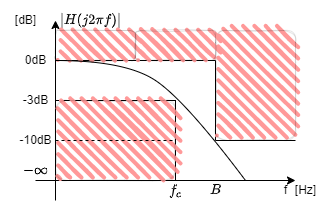
\includegraphics[scale=0.7]{./Images/02Concept/01spesifikasjon.png}
	\caption{Ønsket amplituderespons på system.}
	\label{fig:02ønsketamplituderespons}
\end{figure}
